\documentclass[11pt]{article}
\usepackage[utf8]{inputenc}
\usepackage[T1]{fontenc}
\usepackage{geometry}
\usepackage{hyperref}
\usepackage{graphicx}
\usepackage{enumitem}
\usepackage{titlesec}
\usepackage{fancyhdr}
\usepackage{color}
\usepackage[table]{xcolor}
\usepackage[spanish]{babel}

% Page margins
\geometry{a4paper, margin=1in}

% Header and footer
\pagestyle{fancy}
\fancyhf{}
\fancyhead[L]{\textit{Proyecto Corto 1}}
\fancyhead[R]{\textit{\today}}
\fancyfoot[C]{\thepage}
\renewcommand{\headrulewidth}{0.4pt}

% Date format for entries
\usepackage{datetime}
\newdateformat{logdate}{\twodigit{\THEDAY}~\shortmonthname~\THEYEAR}

% Custom section for log entries
\titleformat{\section}
  {\normalfont\Large\bfseries}
  {Entry \#\thesection:}
  {0.5em}
  {}

% Entry counter
\newcounter{entrycount}
\setcounter{entrycount}{0}

% New log entry command
\newcommand{\logentry}[3]{%
  \refstepcounter{entrycount}%
  \section*{Bitácora \#\theentrycount: #1}%
  \hfill\textit{#2}\\[0.2cm]
  #3
  \vspace{0.5cm}
  \hrule
  \vspace{0.5cm}
}

\begin{document}

% Title
\begin{center}
    {\huge \textbf{Bitácora}}\\[0.3cm]
    {\large \textbf{Proyecto:}} Diseño digital combinacional en dispositivos programables\\[0.2cm]
    {\large \textbf{Repositorio:}} \texttt{https://github.com/jwoc101/Proyecto\_1\-Grupo\_5}\\[0.2cm]
    {\large \textbf{Estudiante:}} Julián Murillo Wo Ching\\[0.2cm]
    {\large \textbf{Carné:}} 2024096679\\[0.2cm]
    {\large \textbf{Grupo:}} 1
\end{center}

\vspace{1cm}
\hrule
\vspace{0.5cm}


\logentry{}{24 de marzo}{
    
    \textbf{Planificación de Receptor:}
    \begin{enumerate}
    
        \item \underline{Módulo decodificador:} 
        	Recibe 7 bits del transmisor. Decodifica, y determina cual bit contiene el error controlado.
        \item \underline{Módulo de corrección:} Recibe los 7 bits del transmisor, y 3 bits adicionales del módulo decodificador. Identifica el error y lo corrige. Manda 4 bits de información correcta al módulo de despliegue en binario y al selector.
        \item \underline{Módulo de despliegue en binario:} Recibe los 4 bits del módulo de corrección y los visualiza mediante los LEDs en la FPGA. 
        \item \underline{Módulo de despliegue en display:} Recibe datos del módulo de despliegue en binario y los códifica en hexadecimal para ser visualizados en un display de 7 segmentos.
        \item \underline{Selector:} Recibe 4 bits del módulo decodificador y 4 bits del módulo de corrección. Mediante un bit adicional que proviene de un switch decide cual de los cuatro bits mandarle al módulo de despliegue en display.

    \end{enumerate}
    
   % \textbf{Observations/Notes:}
    %\begin{itemize}
     %   \item Everything installed smoothly
      %  \item Need to verify configuration tomorrow
    %\end{itemize}
    
\begin{figure}[!ht]
    \centering
    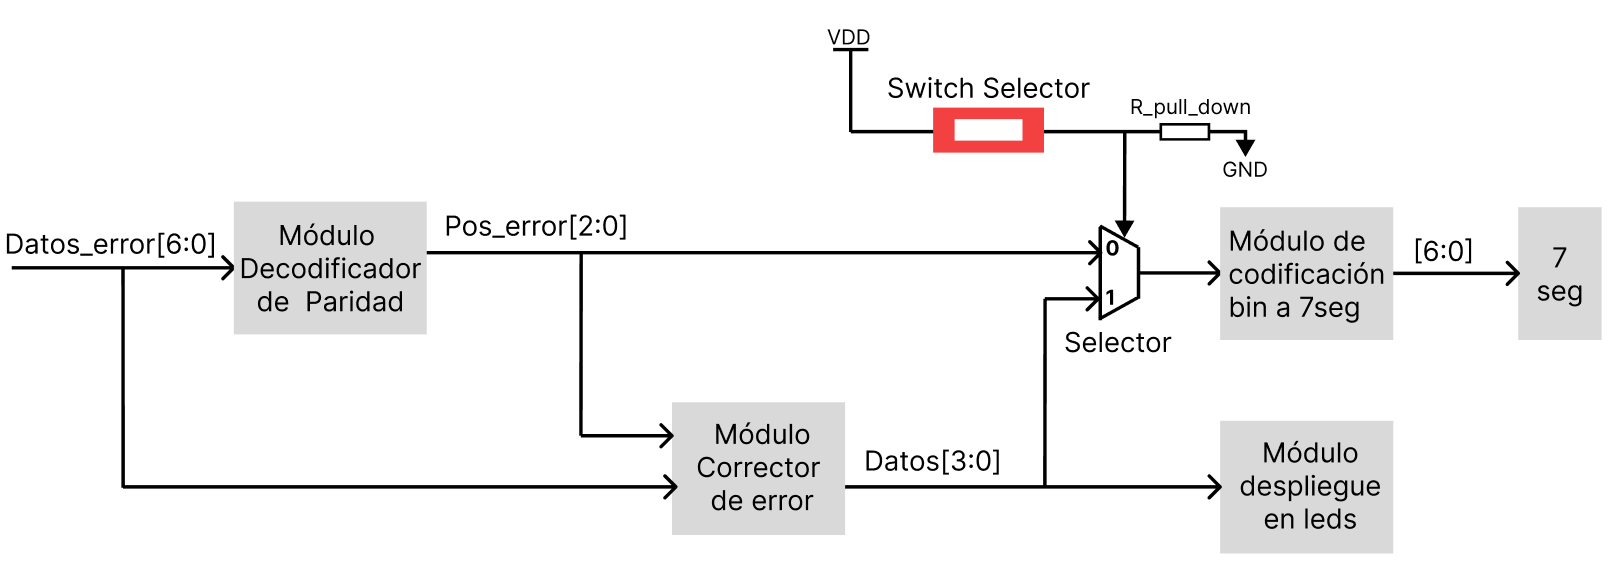
\includegraphics[width=\linewidth]{modulos_receptor_guia.png}
    \caption{Esquema de módulos de receptor}
\end{figure}	    
    
	\vspace{2cm}    
    
    \textbf{Investigar:}
    \begin{itemize}
        \item Algoritmo de Hamming, Hamming (7,4)
        \item Especificaciones y programación en FPGA con SystemVerilog (transmición de datos, visualización con LEDs)
        \item Elaboración de diagramas de bloques para subsistemas
    \end{itemize}
}

\logentry{}{2 de abril}{

	\textbf{Sesión de estudio de Verilog:} Quick Start Guide to Verilog\cite{lameres2024}
	
	Capítulo 2: Módulos, Puertos, Señales, Parámetros, Vectores, Directivas de compilador	
	
	Capítulo 3: Operadores, Asignación Continua
	\\

	
}

\logentry{}{6 de abril}{

	\textbf{Resumen:}
	\begin{itemize}
		\item Sesión de estudio de códigos de corrección Hamming
		\item Sesión de troubleshooting para comando \texttt{make load	}
		\item Pruebas preliminares de programación en el FPGA con módulos de prueba
	\end{itemize}
	
	\vspace{1cm}
	
	\textbf{Sesión de estudio de códigos de corrección Hamming:} 
	
	But what are Hamming codes? The origin of error correction\cite{3B1B2020}
	
	\vspace{1cm}
	
	\textbf{Sesión de Troubleshooting:}
	
	\underline{Problema:} El comando del Makefile \texttt{make load} no estaba abriendo el FPGA a pesar de estar conectado e identificado. Se identificó que el driver \textit{ftdi\_sio} de Archlinux estaba utilizando el FPGA de manera exclusiva y continua. Este driver no permite que la herramienta FPGA obtenga acceso directo al dispositivo USB para programación basada en JTAG.
	
	\underline{Solución:} Se desmontó el driver con el comando: \texttt{sudo rmmod ftdi\_sio }
	
	\vspace{0.5cm}
	
	\underline{Problema:} \texttt{make load} no detectó ningún archivo o directorio llamado openFPGAloader.
	
	\underline{Solución:} Se instaló la herramienta correspondiente con el comando: \texttt{yay -S openfpgaloader}
	\\
	
}

\logentry{}{7 de abril}{

	\textbf{Programación de Módulos}
	\begin{enumerate}
		\item \underline{Módulo decodificador:} decodificador.sv
		
		\item \underline{Módulo de corrección:} corrector.sv
		
		\item \underline{Módulo top de receptor:} receptor.sv
		
		\item \underline{Testbench básico:} receptor\_tb.sv
	\end{enumerate}
	
	\underline{Problema encontrado:} El output proveniente de 4 pins del FPGA no corresponde al resultado deseado. Por ejemplo, para un input de 0000000 se enseña un output de 0100, cuando debería ser 0000 para Hamming(7,4). El testbench parece mostrar que la lógica de los módulos funciona correctamente, por lo que se deduce que el problema está relacionado al hardware. Posibles causas son una mala asignación de pines en los módulos y el archivo de \textit{constraints}, o el uso de pins especiales que no permiten programación. 
	
	\vspace{1cm}
	
	\textbf{Siguientes Pasos}
	
	\begin{itemize}
		\item Resolver problema encontrado
		
		\item Continuar con programación de módulos
	\end{itemize}		
	 
	

}

\logentry{}{11 de abril}{

	\textbf{Alambrado de circuito:}
	
	\begin{itemize}
	\item Se incorporó el display de 7 segmentos a los pines de salida respectivos
	\item Se verificó la funcionalidad de los LEDs incorporados en la FPGA.
	\end{itemize}

\vspace{1cm}

	\textbf{Notas}
	\begin{itemize}
	\item Se descubrió que las LEDs de la FPGA se encienden con un \'cero\' lógico. Se invirtió la entrada del módulo \texttt{led\_display.sv}.
	\item El módulo \texttt{seg7\_display.sv} fue diseñado para un display de ánodo común, pero en la práctica se utilizó uno de cátodo común, por lo que también está invertido.
	\end{itemize}

}

\logentry{}{12 de abril}{

	\textbf{Acciones:}
	\begin{itemize}
	\item Se incorporaron 4 LEDs adicionales al circuito para indicar ya sea el mensaje decodificado, o la posición del error detectado y corregido. 
	\item Se hizo un testbench que prueba todas las entradas posibles con solo un 'uno' lógico en alguna de sus posiciones. También permite añadir fácilmente entradas personalizadas.
	\end{itemize}
	
\vspace{1cm}	
	
	\textbf{Notas:}
	\begin{itemize}
	\item Se carece de un multiplexor de 2 entradas de 4 bits, así como un switch. Por lo tanto, los cuatro LEDs incorporados hoy no cumples con la funcionalidad dual descrita. Por el momento se tienen que conectar manualmente los pines de la palabra, así como los pines de la posición de error, a preferencia. 
	\item Como la palabra decodificada es de 4 bits, pero la posición del error es de 3, hay un LED que no se utiliza al enseñar la posición del error. Este corresponde al del bit más significativo de la palabra corregida en binario. 
	\end{itemize}		
	
}

\logentry{}{13 de abril}{

	\textbf{Reunión con Pareja del Transmisor:}
	\begin{itemize}
	\item Se tuvo que invertir el orden de asignación de los \texttt{wire} de la palabra corregida y la posición del error, convirtiendo sus bits más significativos en los menos significativos y vice versa. Esto se hizo por motivos de funcionalidad con el transmisor. Esta medida solo se tomó para la revisión conjunta, el código en el repositorio no posee esta particularidad.
	\item Se comprobó el funcionamiento exitoso del circuito receptor.
	\end{itemize}

\vspace{1cm}

	\textbf{Acciones Adicionales:}
	\begin{itemize}
	\item Se obtuvo un multiplexor 74ls157, así como un switch. 
	\item Se incorporó exitosamente el módulo selector del circuito.
	\end{itemize}


}


\logentry{}{14 de abril}{

	\textbf{Revisión (Recomendaciones del Asistente):}
	\begin{itemize}
	\item Añadir resistencias de \textit{pull\-down} a los pines de entradada para proteger la FPGA.
	\item Utilizar \texttt{logic} en vez de \texttt{wire} en el código de Verilog para mejor grabado de datos. 
	\end{itemize}

\vspace{1cm}

	\textbf{Siguientes Pasos:}
	\begin{itemize}
	\item Desarrollo de diagramas de bloques para cada subsistema.
	\item Desarrollo de informe del proyecto.
	\end{itemize}

}

	\begin{thebibliography}{99}
	\bibitem{lameres2024}
	B. J. LaMeres, \textit{Quick Start Guide to Verilog}, 2nd ed., Cham, Switzerland: Springer, 2024.
	\bibitem{3B1B2020}
	3Blue1Brown, \textit{But what are Hamming codes? The origin of error correction}, YouTube, 4 de septiembre de 2020. [En línea]. Disponible en: https://www.youtube.com/watch?v=X8jsijhllIA
	\end{thebibliography}
% ------------------------------------------------------------
% Copy this block for each new log entry
% ------------------------------------------------------------
% \logentry{[Entry Title]}{
%     \textbf{Date:} \logdate\today\\
%     \textbf{Time Spent:} [duration]\\
%     \textbf{Category:} [type]\\
%     
%     \textbf{What I did:}
%     \begin{itemize}
%         \item [task 1]
%         \item [task 2]
%     \end{itemize}
%     
%     \textbf{Observations/Notes:}
%     \begin{itemize}
%         \item [observation 1]
%         \item [observation 2]
%     \end{itemize}
%     
%     \textbf{Next Steps:}
%     \begin{enumerate}
%         \item [next action 1]
%         \item [next action 2]
%     \end{itemize}
% }
% ------------------------------------------------------------

\end{document}